\subsection{Programmable Privacy}

Programmability The privacy platform has two main features (1)It supports private 
transactions, not only private transactions. Similar to Zcash \cite{website:Zcash}, users can still 
choose the transaction type, public transaction or private transaction independently; 
(2)Support Programmability, you can deploy any smart contract, public contract or 
private contract, depending on the needs of the project party. Compared with Specific 
Privacy, the main difference is the logic of state transition in Note, from specific 
calculation to arbitrary calculation logic. Figure \ref{fig:Difference between Specific Privacy and Programmable Privacy} simply shows the difference 
between the two.
\begin{figure}[!ht]
    \centering
    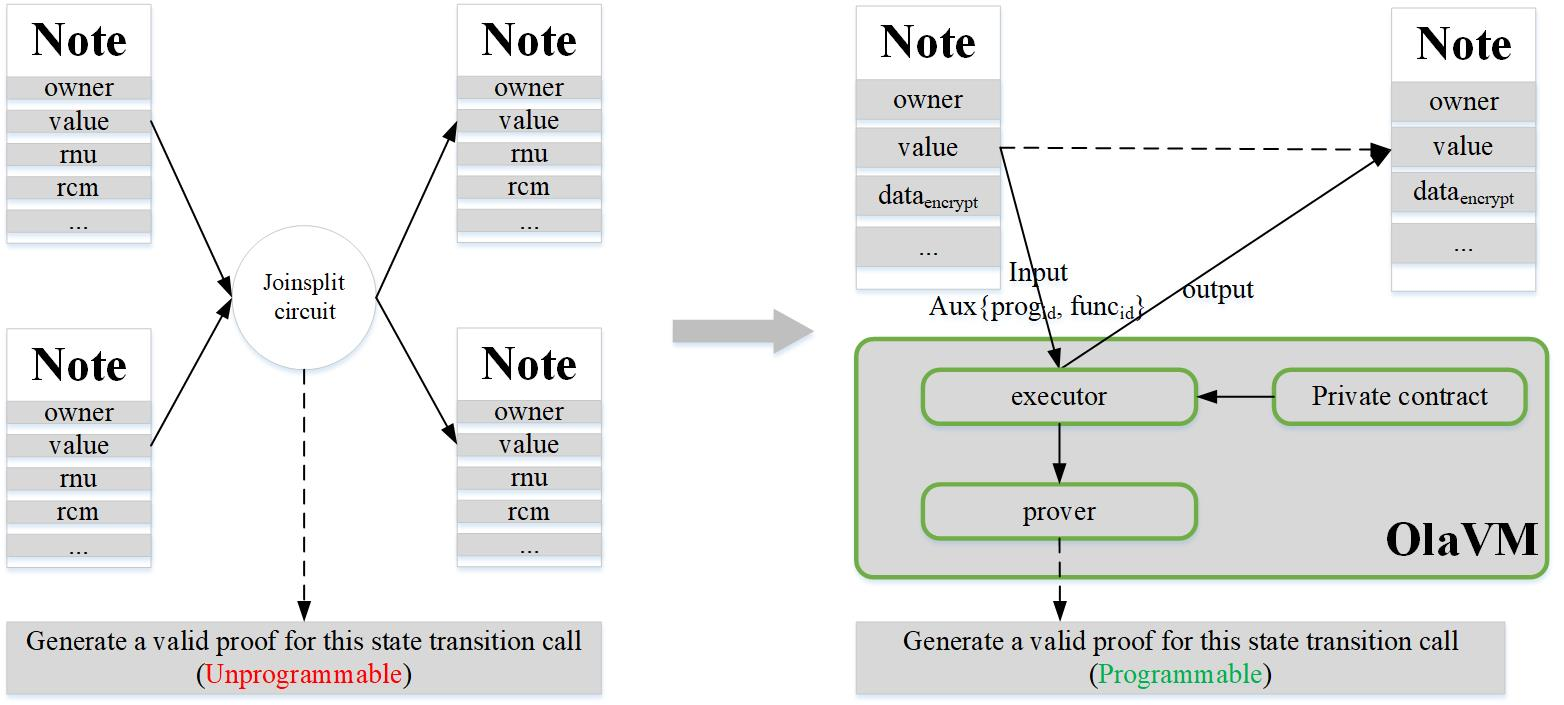
\includegraphics[width=0.6\textwidth]{Difference between Specific Privacy and Programmable Privacy.jpg}
    \caption{Difference between Specific Privacy and Programmable Privacy}
    \label{fig:Difference between Specific Privacy and Programmable Privacy}
\end{figure}

The current projects focusing on programmable privacy are Aleo \cite{website:Aleo} and Aztec \cite{website:Aztec}. Aleo \cite{website:Aleo} is a 
privacy public chain, from BTC \cite{website:BTC} to Ethereum \cite{website:Ethereum} to Zcash \cite{website:Zcash} to Aleo \cite{website:Aleo}. It makes up for 
the fact that programmability and privacy cannot coexist at the Layer1 level. 
It has reached the testnet stage and supports developers to deploy privacy contracts; 
Aztec \cite{website:Aztec} focuses on doing Layer2 programmable privacy for Ethereum \cite{website:Ethereum} , a project 
called Aztec3 \cite{website:Aztec3}, is still in development.

Before we clarify the different approachs to get programmability, we should give some explanations on Domain Specific Language(DSL)  \cite{website:DSL} and General Purpose Language(GPL)  \cite{website:DSL}.
DSL \cite{website:DSL} is defined as: a computer programming language of limited expressiveness focused on a particular domain, limited expressiveness means it just supports a bare minimum of features 
needed to support its domain. You can't build an entire software system in a DSL; rather, you use a DSL \cite{website:DSL} for one particular aspect of a system. While GPL \cite{website:DSL} is defined as: A general-purpose programming language
provides lots of capabilities: suppoting varied data, control, and abstraction structures. For convenience, we call the GPL in blockchain as Smart Contract Language(SCL).

So there are often two ways to achieve programmability, one is design a DSL, such as Circom \cite{website:Circom} , Pil \cite{website:Pil}, Noir \cite{website:Noir}, etc..; the other is SCL, 
such as Cairo1.0 \cite{website:Cairo1.0}, Solidity \cite{website:Solidity}, Ola lang \cite{website:Ola-lang} and so on. Like we have mentioned before, the main difference is that SCL supports more complex structures and has 
higher abstraction, it's more suitable for writing complex business logic and meanwhile, DSL is more suitable for some simple computational expression. 
Take Polygon Hermez's \cite{website:Polygon-Hermez} Pil \cite{website:Pil} language as an example, you can directly use it to define a simple micro-op, such as `A * B + C`, or `A * B * C + D` and other simple combinations. 
Table \ref{table:Difference between DSL and SCL} briefly shows some of the differences between DSL and SCL.

\begin{table}[!ht]
    \centering
    \begin{tabular}{|l|l|l|l|l|l|}
    \hline
        \emph{Type} & \emph{Abstraction} & \emph{Process} & \emph{Difficulty} & \emph{Examples} & \emph{Notes} \\ \hline
        DSL & low & program -> arith-ops -> ops gadgets & normal & \makecell{circom \\ noir \\ cairo} & \makecell{1. semantic analysis \\ 2. codeGen optimization} \\
        \makecell{SCL \\ (ISA/VM)} & high & program -> bytecodes -> cpu circuit & hard & \makecell{solidity \\ cairo1.0 \\ ola lang} & \makecell{1. need a compiler \\2. re-use LLVM framework} \\
    \end{tabular}
    \caption{Difference between DSL and SCL}
    \label{table:Difference between DSL and SCL}
\end{table}

If you want to prove a program written by DSL are executed correctly(this is what ZKDSL means), you may need to predefine some commonly used operators, each corresponding to a circuit, called a Gadget \cite{website:Gadget}; you can use these operators to combine any desired calculation logic and 
encapsulate it into a function, Therefore, each function can be regarded as a specific calculation; but the call and return logic between functions cannot be handled because the op of the function
 call and the corresponding constraints are not handled. And If you want to prove a program written by SCL are executed correctly(this is what ZKVM means), you need design corresponding constraints for each instruction, collectively referred to as cpu circuit; therefore, Any program will be compiled into 
 bytecodes composed of these instructions, and then constrained by the cpu circuit.

Ola chose to implement a customize SCL to get programmability even through it's more harder that DSL, as we could get:
 \begin{itemize}
 \item A higher abstraction and programmable language, allowing developers to write smart contracts with arbitrary logic;
 \item A full-featured zk-friendly VM can be designed to achieve higher system performance;
 \item LLVM-based compiler, can be more easily compatible with other advanced programming languages;
\end{itemize}